\section{Apache Software Foundation}
\label{sec:asf}

\begin{figure}[H]
    \centering
    
\includegraphics[width=0.7\textwidth]{asf-logo.png}
    \caption{Apache Software Foundation Communtity talk by Santiago Gala}
    \label{apache-logo}
\end{figure}

\textit{Apache Software Foundation} - \textbf{ASF} - \href{http://en.wikipedia.org/wiki/501(c)_organization#501.28c.29.283.29}{501.3 epigraph C nonprofit Foundation}

ASF defines itself as:
\begin{quotation}
    \emph{"not simply a group of projects sharing a server, but rather a community of developers and users"}
\end{quotation}

A \textit{Foundation} is a legal umbrella to allow us to legality providing transparency.

\subsection{Volunteers contributions}

\par Apache could be defined as a community of communities. Therefore contributors enter for each community through its rules. The basic rules are inherited and common from ASF.
\\ To make a contribution, first, the contributor must be in contact with the particular community and its ecosystem project.pse, EUPL, FLOSS, FLOSSIE, flos
\\ In Apache projects bear a similarity in ecosystems, because they have been through an acceptance process to be adopted or published by Apache.
\\ As each project is:
\begin{itemize}
	\item \textit{Mailing lists}.
	\item \textit{Source code}.
	\item \textit{Bug tracking}.
	\item \textit{Mentors}.
	\item \textit{Committers}.
	\item \textit{Documentation} (wikis, html, pdf...).
\end{itemize} Therefore, in order to help you to follow the guidelines set. It is recommended in all FLOSS projects you can register for mailing lists as a first step to find out how it works and basic communication. Then begin to understand the design, installation, use and testing.
\\ You can read a summary of the basic rules for contributors http://www.apache.org/dev/contributors.html ASF.
\\ For becoming a contributor, you have to be invited by the other contributors of the project. Having won merits and respect within the community.

\subsection{How to Contribute}

\par If you want to become a contributor in a project at Apache Software Foundation, a tip, you could start following \href{http://incubator.apache.org/}{incubator projects}.

\begin{figure}[htp]
    \centering
    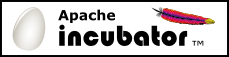
\includegraphics[width=0.7\textwidth]{egg-logo.png}
    \caption{Apache Incubator}
    \label{egg-logo}
\end{figure}

\par For a project, this is the previous step before become an Apache project. These projects are looking for create a hudge community and it's easier to become a contributor than in bigger projects from ASF.

\par Every new committer must read Apache Software Foundation Guide introducing all aspects that are needed for a committer:

\begin{itemize}
	\item \textit{Contributor License Agreement} - to contribute with your commits to ASF.
	\item \textit{Account creation} - step by step using ASF standards.
	\item \textit{Responsibilities} - as a member of ASF, personal web space, community, ApacheCon.
\end{itemize} You can find an extense explanation in \href{http://www.apache.org/dev/new-committers-guide.html}{ASF new committers guide}.

\subsection{Committers resources}

\par An interesting link of how decisions are made in the Apache Software Foundations to see meritocracy in action:
\begin{itemize}
	\item \url{http://community.apache.org/committers/}
\end{itemize}

% section  (end)